\documentclass[t,xcolor={dvipsnames}]{beamer}

\usepackage{pgfpages}

\usetheme{metropolis}

%\setbeameroption{show notes on second screen=right}
%\setbeamertemplate{note page}{\pagecolor{white}\insertnote}

\usepackage{palatino}

\usepackage[utf8]{inputenc}
\usepackage[T1]{fontenc}
\usepackage[ngerman]{babel}
\usepackage[autostyle=true]{csquotes}
\usepackage{booktabs}
\usepackage{tikz}
\usepackage{pgfplots}
\usetikzlibrary{patterns,shapes.arrows}
\usetikzlibrary{calc,positioning,fit}%
\usepgfplotslibrary{groupplots,dateplot}
\pgfplotsset{compat=newest}
\usepackage{mathtools}
%\usepackage{lmodern}
\usepackage{subfloat}
\usepackage{subcaption}
\usepackage{enumitem}
\DeclarePairedDelimiter\abs{\lvert}{\rvert}
\usepackage{pgfplots}
\usepackage{siunitx}
\sisetup{locale = DE}
\sisetup{table-auto-round = true}

\usepackage{wasysym}
\renewcommand{\qedsymbol}{\mbox{\ooalign{$\smiley$\cr\hidewidth$\square$\hidewidth\cr}}}

\usepackage{amsthm}
\theoremstyle{definition}
\newtheorem{conjecture}{Vermutung}

%%%

\title{Anwendung von Contraction Hierarchies und Hierarchical Hub-Labeling auf Geometrischen Graphen}
\author{Christian Wilhelm Staib}
\institute{Abschlusspräsentation Bachelorarbeit \\ Universität Stuttgart}
\date{22.10.2024}

%%%

\begin{document}

\begin{frame}
    \maketitle
\end{frame}

%%%

\begin{frame}{Übersicht}
    \begin{enumerate}[label = \arabic*)]
        \item
              Problemstellung

        \item
              Überlegungen zur Kontraktion

        \item
              PEOPLE
    \end{enumerate}
\end{frame}

%%%

\begin{frame}{Problemstellung}
    \begin{figure}
        \centering
        \begin{tikzpicture}[scale=1]
            % Variablen für das erste Polygon
            \coordinate (a0) at (0.5,0+0.2);
            \coordinate (a1) at (1,2+0.2);
            \coordinate (a2) at (2,1+0.2);
            \coordinate (a3) at (1.5,0+0.2);

            \filldraw (a0) circle (2pt);
            \filldraw (a1) circle (2pt);
            \filldraw (a2) circle (2pt);
            \filldraw (a3) circle (2pt);

            % Zeichne das erste Polygon
            \draw[thick] (a0) -- (a1) -- (a2) -- (a3) -- cycle;
            \node at (a0) [below left] {$s$};

            % Variablen für das Rechteck in der Mitte
            \coordinate (b0) at (4,0);
            \coordinate (b1) at (4,3);
            \coordinate (b2) at (5,3);
            \coordinate (b3) at (5,0);

            \filldraw (b0) circle (2pt);
            \filldraw (b1) circle (2pt);
            \filldraw (b2) circle (2pt);
            \filldraw (b3) circle (2pt);

            % Zeichne das Rechteck in der Mitte
            \draw[thick] (b0) -- (b1) -- (b2) -- (b3) -- cycle;


            % Variablen für das letzte Polygon
            \coordinate (c0) at (7,0+0.35);
            \coordinate (c1) at (8,1+0.35);
            \coordinate (c2) at (7.5,2+0.35);
            \coordinate (c3) at (6.5,1.5+0.35);

            \filldraw (c0) circle (2pt);
            \filldraw (c1) circle (2pt);
            \filldraw (c2) circle (2pt);
            \filldraw (c3) circle (2pt);

            % Zeichne das letzte Polygon
            \draw[thick] (c0) -- (c1) -- (c2) -- (c3) -- cycle;

            \node at (c2) [above right] {$t$};

            \draw[dashed] (a1) -- (b0);
            \draw[dashed] (a1) -- (b1);

            \draw[dashed] (a2) -- (b0);
            \draw[dashed] (a2) -- (b1);

            \draw[dashed] (a3) -- (b0);
            \draw[dashed] (a3) -- (b1);

            \draw[dashed] (b2) -- (c0);
            \draw[dashed] (b2) -- (c2);
            \draw[dashed] (b2) -- (c3);

            \draw[dashed] (b3) -- (c0);
            \draw[dashed] (b3) -- (c3);
        \end{tikzpicture}
        \caption{Beispiel Euclidean Shortest Path Problem}
    \end{figure}
\end{frame}

\begin{frame}{Problemstellung}
    \begin{figure}[h!]%
        \centering
        \subfloat[\centering{}aegaeis-graph]{{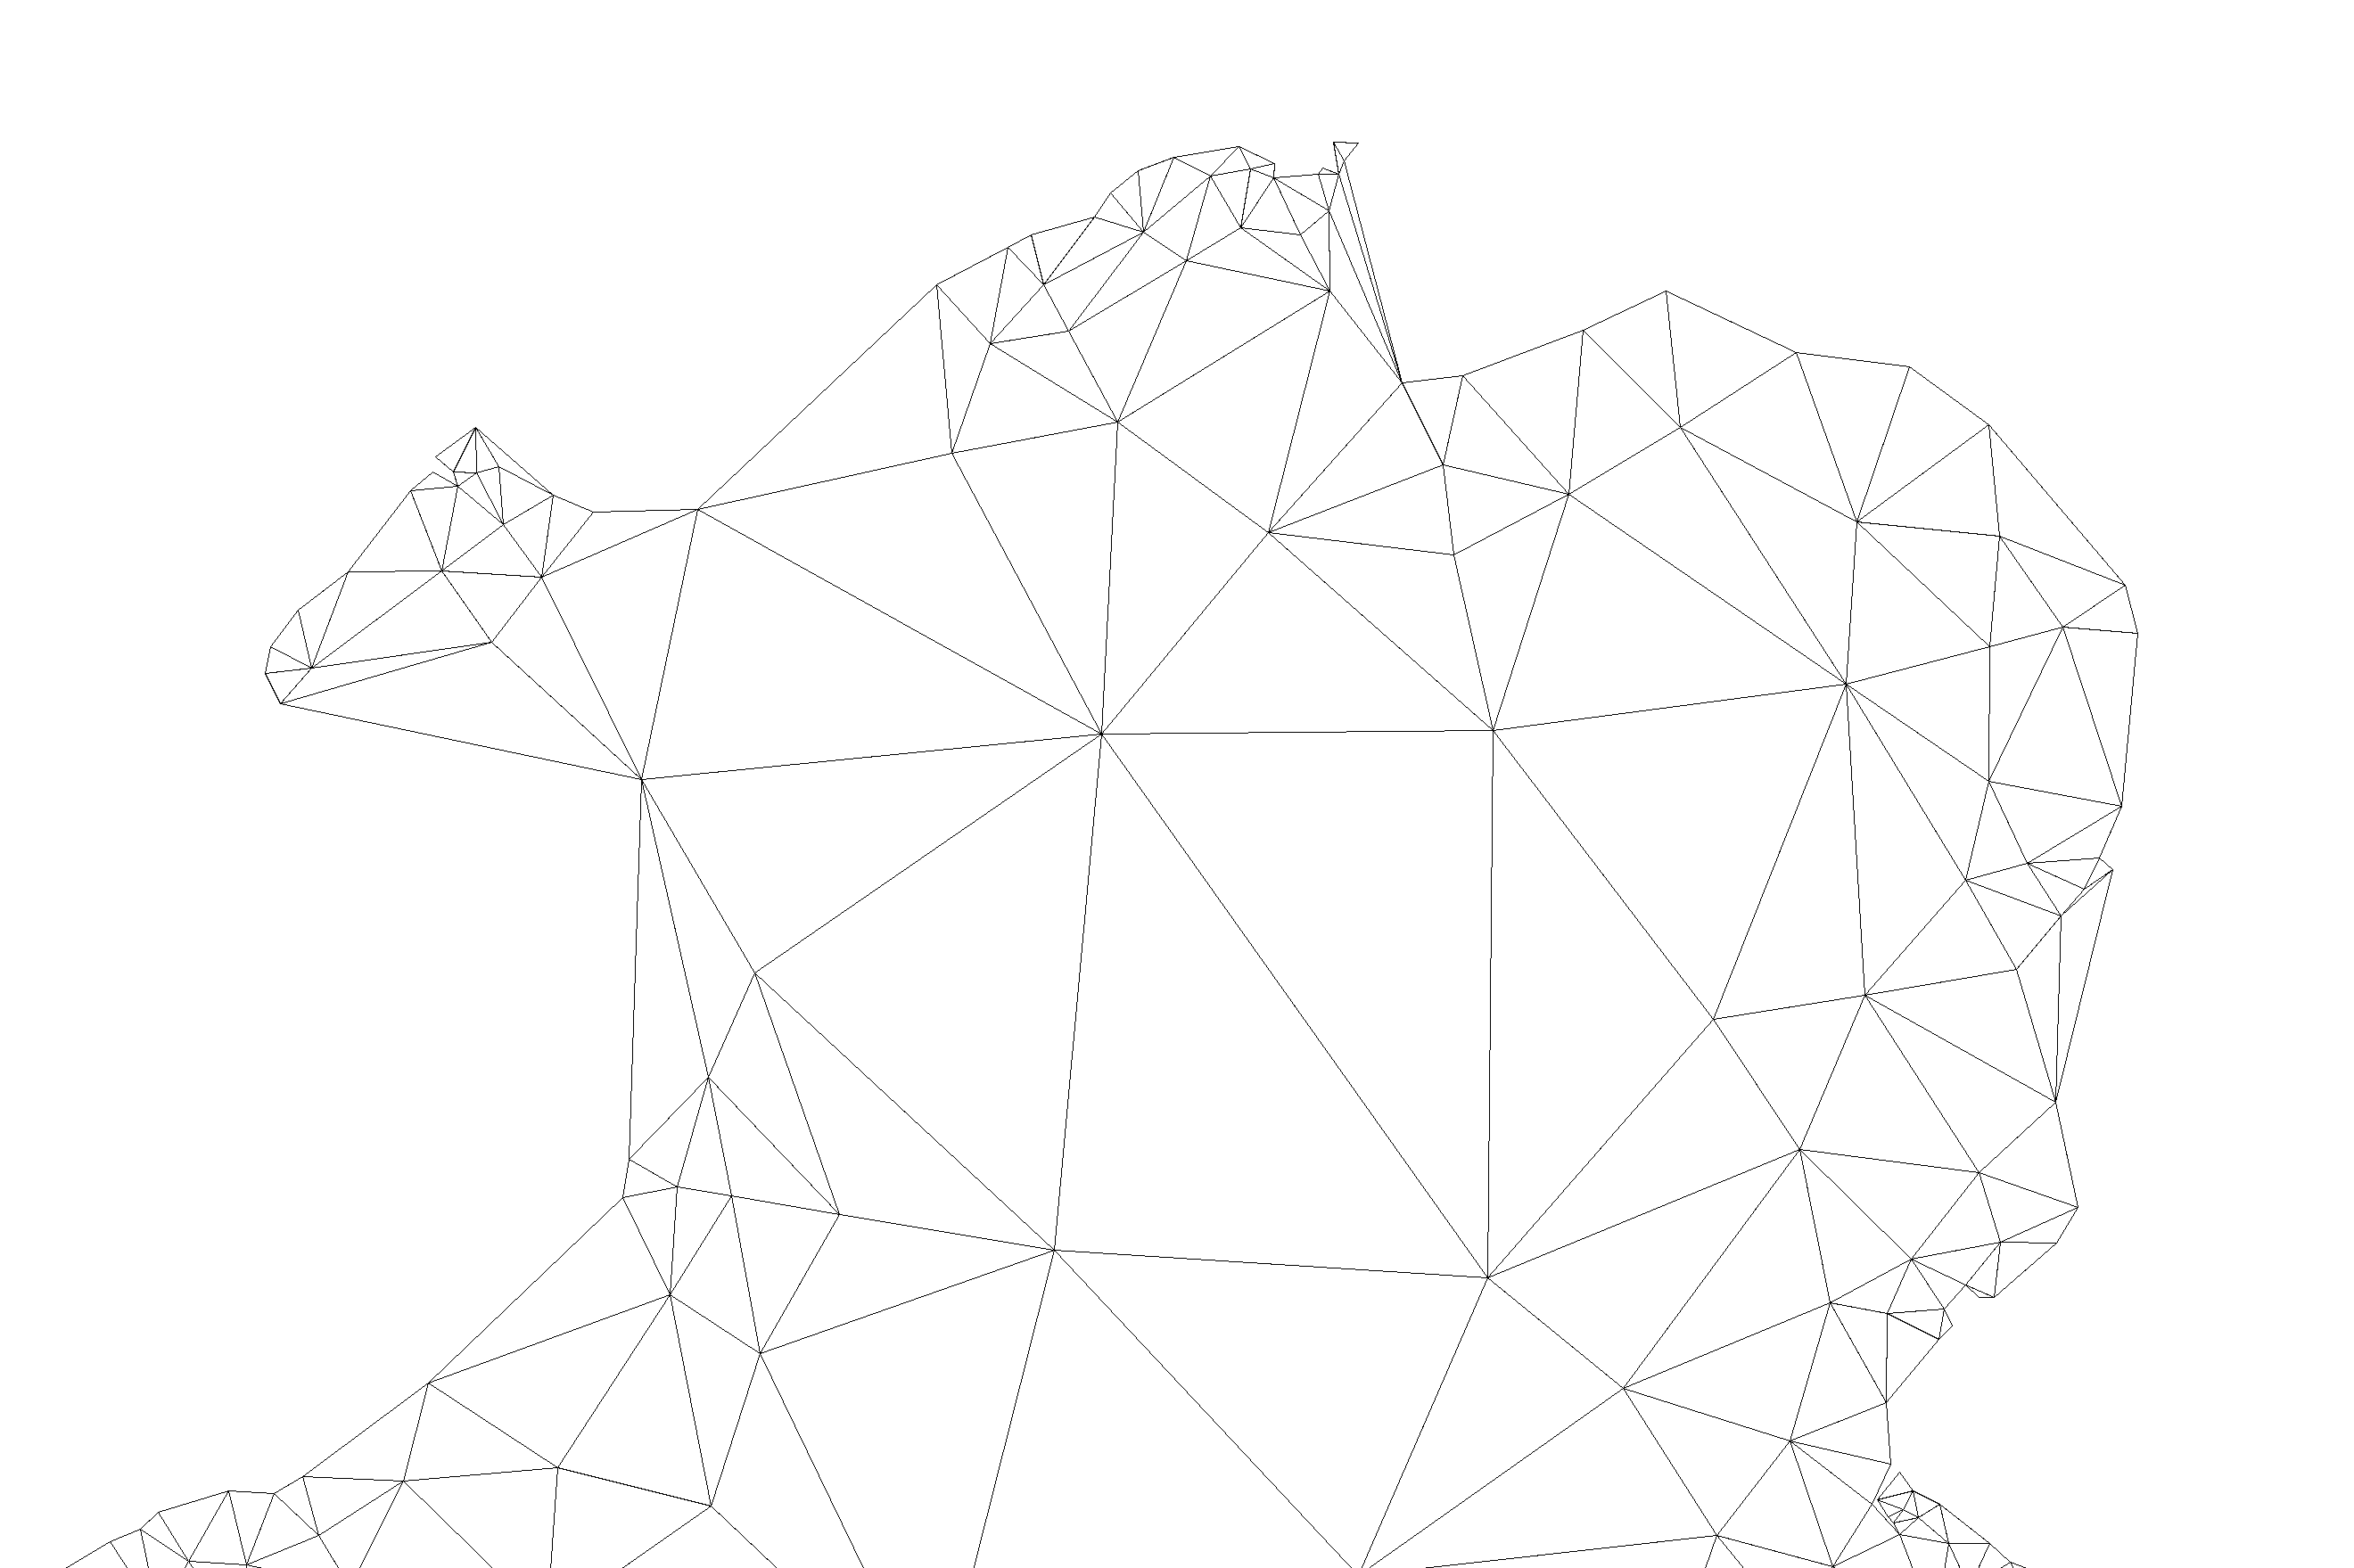
\includegraphics[width=.5\linewidth - 0.25cm]{img/thessaloniki-graph.png} }}%
        %\qquad
        \subfloat[\centering{}aegaeis-visibility]{{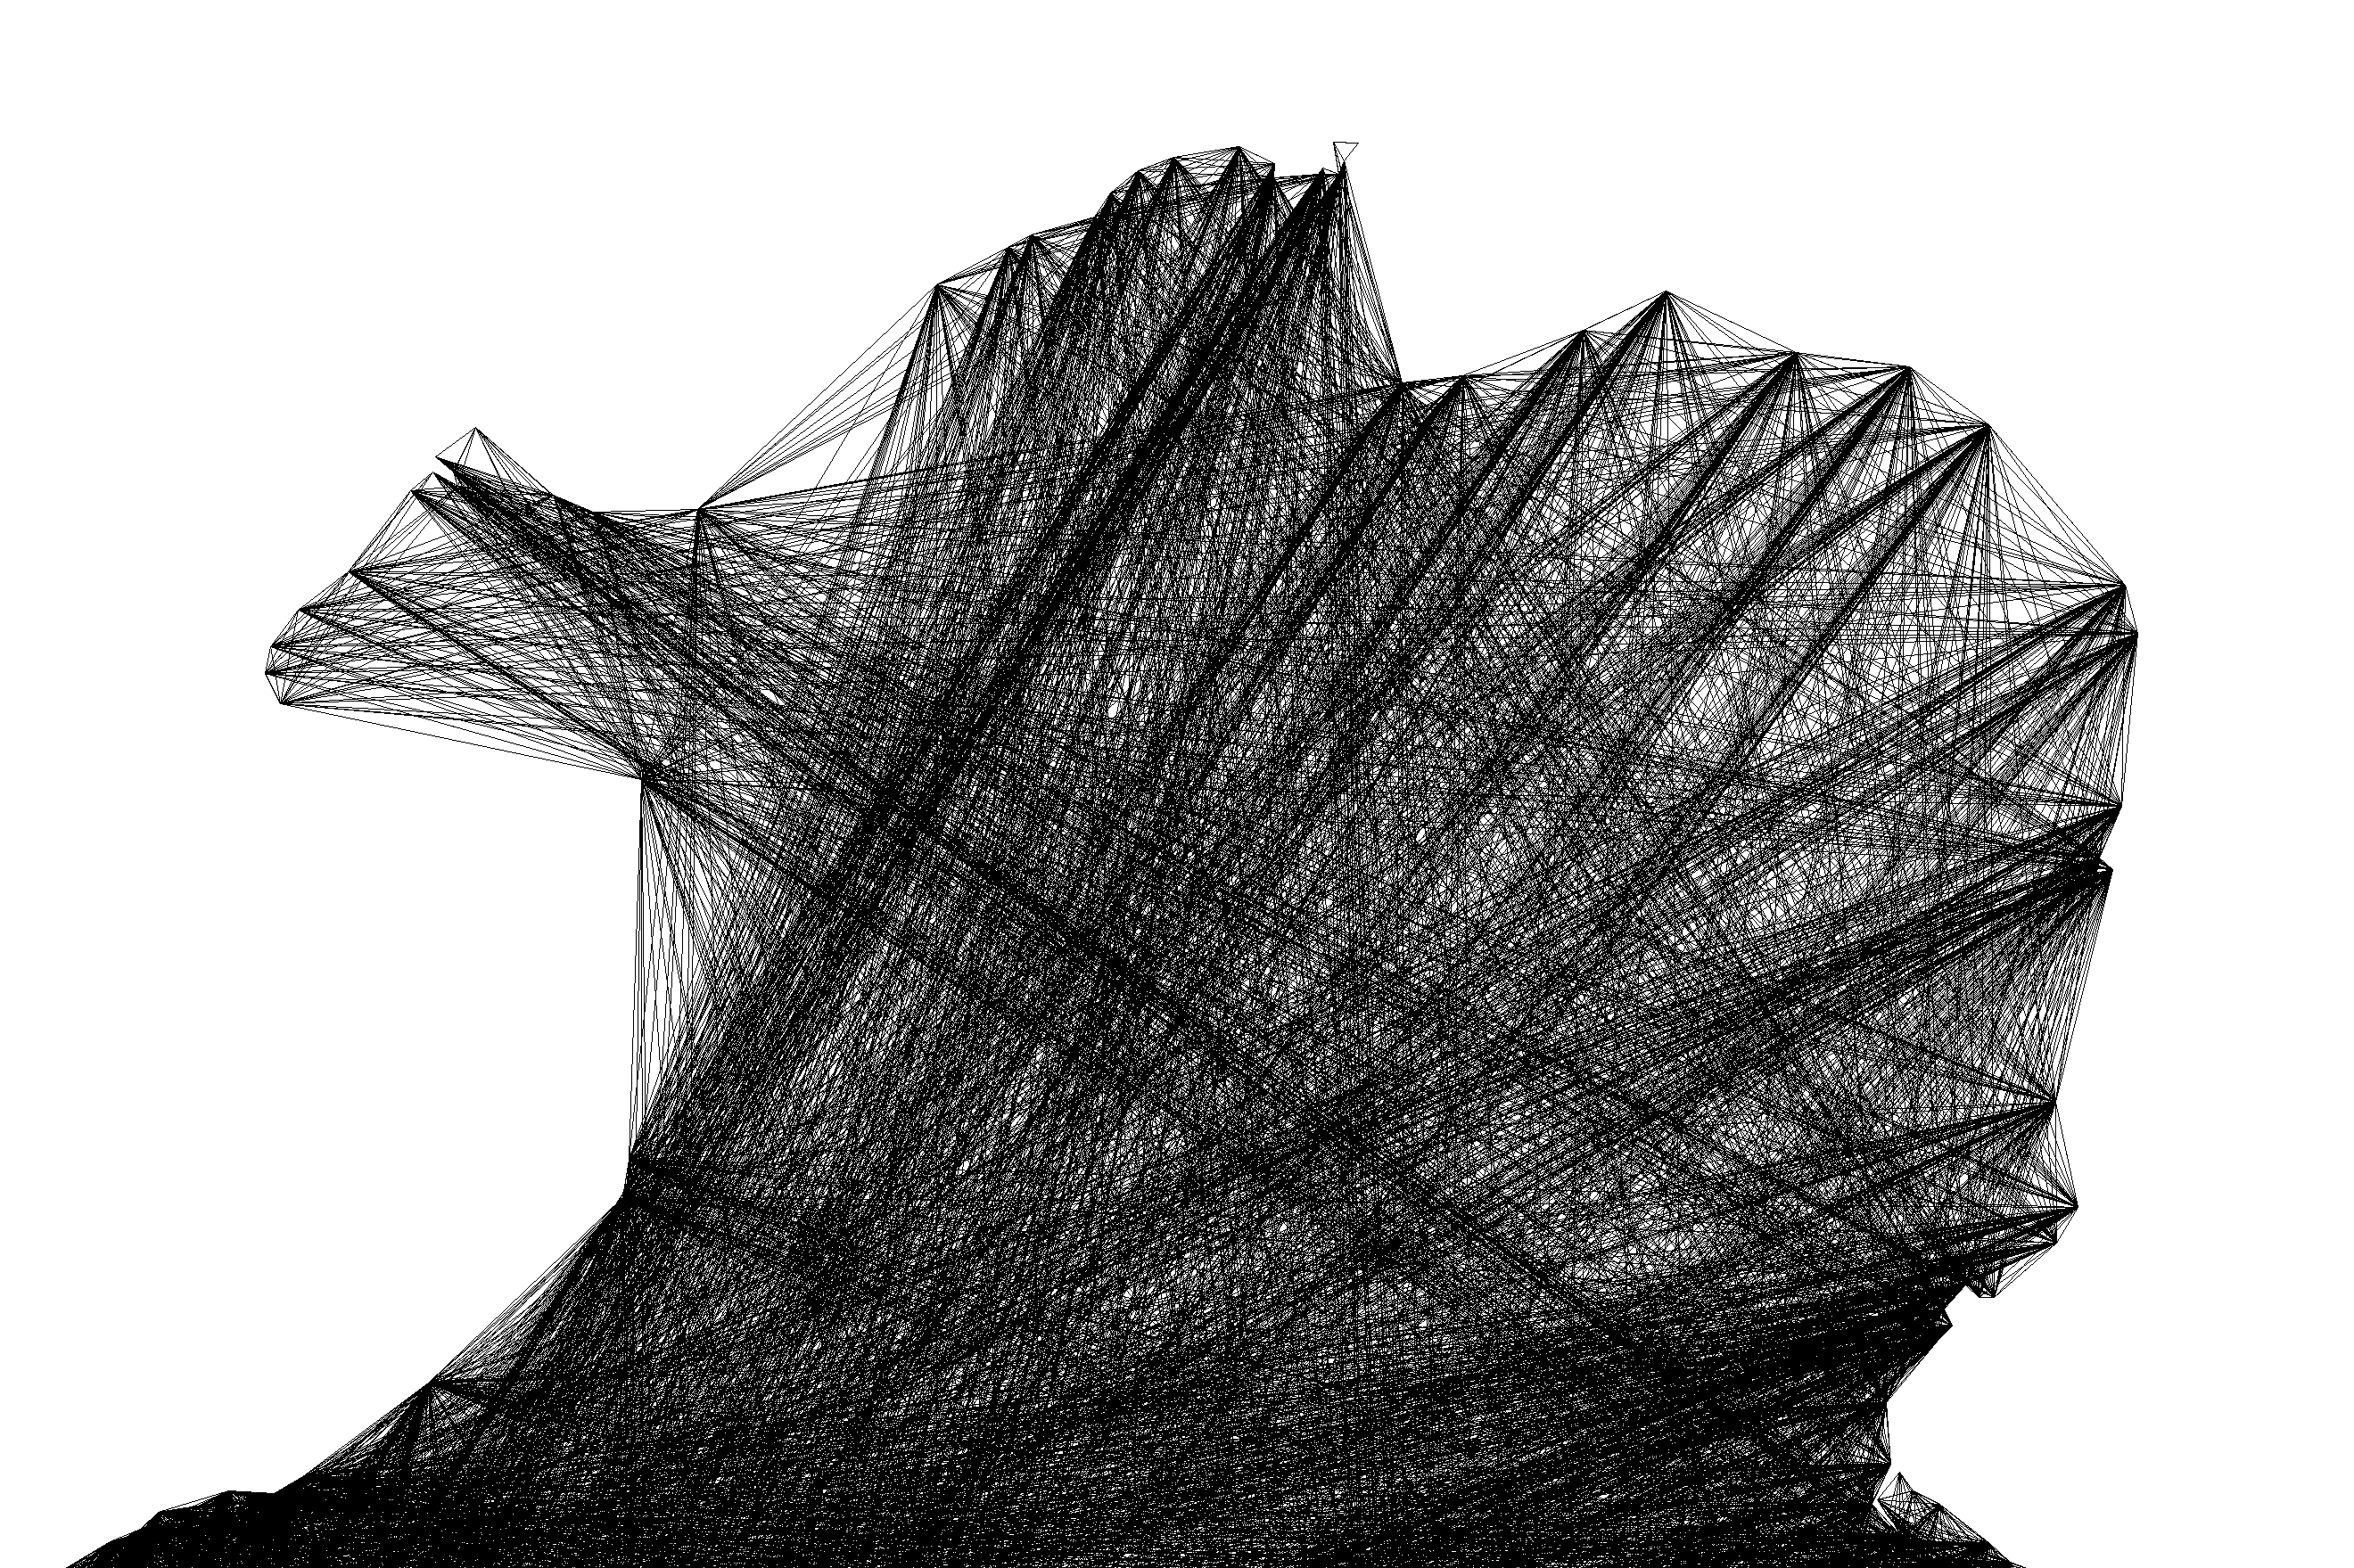
\includegraphics[width=.5\linewidth - 0.25cm]{img/thessaloniki-visibility.png} }}%
        \caption{Hafen von Thessaloniki}%
        \label{fig:thessaloniki_comparison}%
    \end{figure}
\end{frame}

\begin{frame}{Problemstellung}

    \begin{table}[h!]
        \centering
        \resizebox{\columnwidth}{!}{%
            \begin{tabular}{
                    l % Graph
                    S[table-format = 7.0] % Zeit
                    S[table-format = 9.0] % Zeit
                    S[table-format = 4.1] % Zeit
                }
                \toprule
                {Graph}                  & {\# Knoten} & {\# Kanten} & {$\varnothing$ Grad}       \\ \midrule
                aegaeis-graph            & 524881      & 2795322     & \fpeval{2795322/524881}    \\
                aegaeis-visibility       & 201040      & 310231834   & \fpeval{310231834/201040}  \\
                medi-graph               & 795606      & 4223566     & \fpeval{4223566/795606}    \\
                medi-visibility          & 310116      & 730772548   & \fpeval{730772548/310116}  \\
                pata-graph               & 2240339     & 11632900    & \fpeval{11632900/2240339}  \\
                pata-visibility          & 1002235     & 315653892   & \fpeval{315653892/1002235} \\
                planet-shrunk-visibility & 188030      & 173385124   & \fpeval{173385124/188030}  \\
                \bottomrule
            \end{tabular}
        }
        \caption{Bearbeitete Graphen}
        \label{table:input_graphs}
    \end{table}
\end{frame}

\begin{frame}{Problemstellung}
    \begin{table}[h!]
        \centering
        \resizebox{\columnwidth}{!}{%
            \begin{tabular}{
                    l % Graph
                    S[table-format = 4.1] % Zeit
                    S[table-format = 3.0] % hop-länge
                    S[table-format = 7.0] % rank
                    S[table-format = 7.0] % queue pops
                }
                \toprule
                {Graph}                  & {$\varnothing$ $t({spd})$} & {$\varnothing$  Hop-Länge} & {$\varnothing$ Dijkstra-Rank} & {$\varnothing$ Queue-Pops} \\
                                         & {(\si{\ms})}               &                            &                               &                            \\
                \midrule
                aegaeis-graph            & 60.281198                  & 215.7201                   & 260447.36                     & 325845.56                  \\
                aegaeis-visibility       & 630.434928                 & 16.311                     & 98650.82                      & 517346.63                  \\
                medi-graph               & 87.08376                   & 340.445                    & 394855.78                     & 494553.97                  \\
                medi-visibility          & 1279.67479                 & 23.6149                    & 154092.42                     & 959206.4                   \\
                pata-graph               & 265.825771                 & 883.979                    & 1120841.9                     & 1387047.8                  \\
                pata-visibility          & 1017.695977                & 63.817                     & 498570.2                      & 2429689.8                  \\
                planet-shrunk-visibility & 529.377185                 & 22.3786                    & 95053.74                      & 691017.2                   \\
                \bottomrule
            \end{tabular}
        }
        \caption{Kennwerte der Dijkstra-Suchen}
        \label{fig:ergebnisse:dijkstra}
    \end{table}
\end{frame}

\begin{frame}{Überlegungen zur Kontraktion}
    \begin{enumerate}[label = \arabic*)]
        \item
              Obere Schranke statt Witness-Suche

        \item
              Hoher Knotengrad macht Kontraktion teuer

        \item
              Bottom-Up aufwändig

        \item
              Parallele Datenstruktur wichtig
    \end{enumerate}
\end{frame}

\begin{frame}{PEOPLE}
    \textbf{P}r\textbf{E}determined \textbf{O}rder, \textbf{P}runed \textbf{L}ab\textbf{e}l

    \begin{figure}[h!]
        \centering
        \begin{tikzpicture}[scale=1.75]
            \node[circle, draw, minimum size=0.6cm, inner sep=0pt , align=center] at (0*1.25, 0) (u) {u};
            \node[circle, draw, minimum size=0.6cm, inner sep=0pt , align=center] at (1*1.25, 0) (v) {v};
            \node[circle, draw, minimum size=0.6cm, inner sep=0pt , align=center] at (2*1.25, 0) (w) {w};

            \draw[->] (u) edge[bend left=45] node[circle, fill=white] {2} (w);
            \draw[->] (u) edge node[circle, fill=white] {1} (v);
            \draw[->] (v) edge node[circle, fill=white] {1} (w);
        \end{tikzpicture}
        \caption{Beispiel Knoten-Kontraktion}
        \label{fig:people:notwendige_kanten}
    \end{figure}
\end{frame}

\begin{frame}{PEOPLE}
    \begin{figure}[h!]
        \centering
        \resizebox{0.7\columnwidth}{!}{%
            \begin{tikzpicture}[]
                % Nodes
                % a & b & c & d & e & f & g & h & i & j & k &
                % 8 & 7 & 3 & 6 & 2 & 5 & 1 & 4 & 0 & 10 & 9 &

                \node[circle, draw, minimum size=1.3cm, inner sep=0pt , align=center] at (2* 1, 0) (a) {a\\8 8};
                \node[circle, draw, minimum size=1.3cm, inner sep=0pt , align=center] at (2* 0, 4) (b) {b\\7 8};
                \node[circle, draw, minimum size=1.3cm, inner sep=0pt , align=center] at (2* 1, 6) (c) {c\\3 10};
                \node[circle, draw, minimum size=1.3cm, inner sep=0pt , align=center] at (2* 1, 8) (d) {d\\6 10};
                \node[circle, draw, minimum size=1.3cm, inner sep=0pt , align=center] at (2* 2, 9) (e) {e\\2 10};
                \node[circle, draw, minimum size=1.3cm, inner sep=0pt , align=center] at (2* 3, 10) (f) {f\\5 10};
                \node[circle, draw, minimum size=1.3cm, inner sep=0pt , align=center] at (2* 3, 7) (g) {g\\1 10};
                \node[circle, draw, minimum size=1.3cm, inner sep=0pt , align=center] at (2* 1, 2) (h) {h\\4 8};
                \node[circle, draw, minimum size=1.3cm, inner sep=0pt , align=center] at (2* 2, 1) (i) {i\\0 8};
                \node[circle, draw, minimum size=1.3cm, inner sep=0pt , align=center, very thick] at (2* 2, 3) (j) {j\\10 10};
                \node[circle, draw, minimum size=1.3cm, inner sep=0pt , align=center] at (2* 2, 5) (k) {k\\9 10};

                \draw[->] (a) edge (b);
                \draw[->] (a) edge (h);
                \draw[->] (a) edge (i);
                \draw[->] (j) edge (c);
                \draw[->] (i) edge (j);
                \draw[->] (k) edge (d);
                \draw[->] (j) edge (k);
                \draw[->] (k) edge (e);
                \draw[->] (k) edge (f);
                \draw[->] (j) edge (g);

                \draw[->] (-2, 0) -- (-2, 10) node[above] {Zeitpunkt der Expansion};

                \draw (-2.5, 4.5) -- (-1.5, 4.5) node[left=1cm] {Abbruch möglich};

            \end{tikzpicture}
        }
        \caption{Contracted-Graph PEOPLE Suchbaum}
        \label{ch:fig:ch_brute_force_suchbaum}
    \end{figure}
\end{frame}

\begin{frame}{PEOPLE}
    \begin{table}[h!]
        \centering
        \resizebox{\columnwidth}{!}{%
            \begin{tabular}{
                    l % Graph
                    r % S[table-format = 4.0] % Erstellung
                    S[table-format = 1.2] % Abkürzungen/Katen
                    S[table-format = 3.2] % average time spd
                    S[table-format = 3.2] % speedup
                }
                \toprule
                {Graph}            & {Erstellung} & {$\frac{\text{Abkürzungen} (C)}{\text{Kanten} (G)}$} & {$\varnothing$ $t({spd})$} & {Speedup}                       \\
                {}                 & {}           & {}                                                   & {(\si{\ms})}               & {}                              \\ \midrule
                aegaeis-graph      & 20m          & \fpeval{12443056/2795322}                            & 2.290886                   & \fpeval{60.281198/2.290886}     \\
                aegaeis-visibility & 5h 53m       & \fpeval{214987558/310231834}                         & 408.948758                 & \fpeval{630.434928/408.948758}  \\
                medi-graph         & 38m          & \fpeval{20003908/4223566}                            & 3.38788                    & \fpeval{87.08376/3.38788}       \\
                medi-visibility    & 20h 52m      & \fpeval{468641256/730772544}                         & 832.555567                 & \fpeval{1279.67479/832.555567}  \\
                pata-graph         & 5h 42m       & \fpeval{70624466/11632900}                           & 10.16729                   & \fpeval{265.825771/10.16729}    \\
                pata-visibility    & 1d 20h 45m   & \fpeval{613324174/315653758}                         & 288.514849                 & \fpeval{1017.695977/288.514849} \\  \bottomrule
            \end{tabular}
        }
        \caption{Kennwerte von mit CH-PEOPLE erzeugten Contracted-Graphen}
        \label{table:ergebnisse:people_ch_speedup}
    \end{table}
\end{frame}


\begin{frame}{PEOPLE}
    \begin{figure}
        \centering
        \resizebox{0.7\columnwidth}{!}{%
            \begin{tikzpicture}
                \begin{axis}[
                        tick align=outside,
                        tick pos=left,
                        x grid style={darkgray176},
                        xlabel={Gesehene Knoten (\%)},
                        xmin=-5, xmax=105,
                        xtick style={color=black},
                        xtick={-20,0,20,40,60,80,100,120},
                        xticklabels={\ensuremath{-}20,0,20,40,60,80,100,120},
                        y grid style={darkgray176},
                        ylabel={Anteil aller Suchen (\%)},
                        ymin=0, ymax=0.910038275342993,
                        ytick style={color=black},
                        ytick={0,0.1,0.2,0.3,0.4,0.5,0.6,0.7,0.8},
                        yticklabels={0,10,20,30,40,50,60,70,80}
                    ]
                    \draw[pattern=north east lines, pattern color=CadetBlue] (axis cs:0,0) rectangle (axis cs:1,0.866703119374279);
                    \draw[pattern=north east lines, pattern color=CadetBlue] (axis cs:1,0) rectangle (axis cs:2,0.0200159655236347);
                    \draw[pattern=north east lines, pattern color=CadetBlue] (axis cs:2,0) rectangle (axis cs:3,0.00872769256270434);
                    \draw[pattern=north east lines, pattern color=CadetBlue] (axis cs:3,0) rectangle (axis cs:4,0.00569271892105661);
                    \draw[pattern=north east lines, pattern color=CadetBlue] (axis cs:4,0) rectangle (axis cs:5,0.00354556556629393);
                    \draw[pattern=north east lines, pattern color=CadetBlue] (axis cs:5,0) rectangle (axis cs:6,0.00217382606724403);
                    \draw[pattern=north east lines, pattern color=CadetBlue] (axis cs:6,0) rectangle (axis cs:7,0.00153939654893376);
                    \draw[pattern=north east lines, pattern color=CadetBlue] (axis cs:7,0) rectangle (axis cs:8,0.00157369003640984);
                    \draw[pattern=north east lines, pattern color=CadetBlue] (axis cs:8,0) rectangle (axis cs:9,0.00189185739243969);
                    \draw[pattern=north east lines, pattern color=CadetBlue] (axis cs:9,0) rectangle (axis cs:10,0.00180421848000012);
                    \draw[pattern=north east lines, pattern color=CadetBlue] (axis cs:10,0) rectangle (axis cs:11,0.00173372631129898);
                    \draw[pattern=north east lines, pattern color=CadetBlue] (axis cs:11,0) rectangle (axis cs:12,0.00117359934918704);
                    \draw[pattern=north east lines, pattern color=CadetBlue] (axis cs:12,0) rectangle (axis cs:13,0.000939260518099339);
                    \draw[pattern=north east lines, pattern color=CadetBlue] (axis cs:13,0) rectangle (axis cs:14,0.00104785656177431);
                    \draw[pattern=north east lines, pattern color=CadetBlue] (axis cs:14,0) rectangle (axis cs:15,0.0013622135303063);
                    \draw[pattern=north east lines, pattern color=CadetBlue] (axis cs:15,0) rectangle (axis cs:16,0.00103452020553341);
                    \draw[pattern=north east lines, pattern color=CadetBlue] (axis cs:16,0) rectangle (axis cs:17,0.00116026299294614);
                    \draw[pattern=north east lines, pattern color=CadetBlue] (axis cs:17,0) rectangle (axis cs:18,0.000956407261837655);
                    \draw[pattern=north east lines, pattern color=CadetBlue] (axis cs:18,0) rectangle (axis cs:19,0.00076779308071806);
                    \draw[pattern=north east lines, pattern color=CadetBlue] (axis cs:19,0) rectangle (axis cs:20,0.000855431993157407);
                    \draw[pattern=north east lines, pattern color=CadetBlue] (axis cs:20,0) rectangle (axis cs:21,0.000737309980739287);
                    \draw[pattern=north east lines, pattern color=CadetBlue] (axis cs:21,0) rectangle (axis cs:22,0.00110691756798331);
                    \draw[pattern=north east lines, pattern color=CadetBlue] (axis cs:22,0) rectangle (axis cs:23,0.000672533393284103);
                    \draw[pattern=north east lines, pattern color=CadetBlue] (axis cs:23,0) rectangle (axis cs:24,0.000544885412122498);
                    \draw[pattern=north east lines, pattern color=CadetBlue] (axis cs:24,0) rectangle (axis cs:25,0.00051821269964103);
                    \draw[pattern=north east lines, pattern color=CadetBlue] (axis cs:25,0) rectangle (axis cs:26,0.000615377580823528);
                    \draw[pattern=north east lines, pattern color=CadetBlue] (axis cs:26,0) rectangle (axis cs:27,0.000802086568194471);
                    \draw[pattern=north east lines, pattern color=CadetBlue] (axis cs:27,0) rectangle (axis cs:28,0.000603946418331835);
                    \draw[pattern=north east lines, pattern color=CadetBlue] (axis cs:28,0) rectangle (axis cs:29,0.000977364393072833);
                    \draw[pattern=north east lines, pattern color=CadetBlue] (axis cs:29,0) rectangle (axis cs:30,0.00054679060587115);
                    \draw[pattern=north east lines, pattern color=CadetBlue] (axis cs:30,0) rectangle (axis cs:31,0.000417237430961115);
                    \draw[pattern=north east lines, pattern color=CadetBlue] (axis cs:31,0) rectangle (axis cs:32,0.000918303386863828);
                    \draw[pattern=north east lines, pattern color=CadetBlue] (axis cs:32,0) rectangle (axis cs:33,0.00080780214944054);
                    \draw[pattern=north east lines, pattern color=CadetBlue] (axis cs:33,0) rectangle (axis cs:34,0.000621093162069708);
                    \draw[pattern=north east lines, pattern color=CadetBlue] (axis cs:34,0) rectangle (axis cs:35,0.000703016493262987);
                    \draw[pattern=north east lines, pattern color=CadetBlue] (axis cs:35,0) rectangle (axis cs:36,0.000459151693431914);
                    \draw[pattern=north east lines, pattern color=CadetBlue] (axis cs:36,0) rectangle (axis cs:37,0.000994511136811038);
                    \draw[pattern=north east lines, pattern color=CadetBlue] (axis cs:37,0) rectangle (axis cs:38,0.000455341305934609);
                    \draw[pattern=north east lines, pattern color=CadetBlue] (axis cs:38,0) rectangle (axis cs:39,0.000497255568405519);
                    \draw[pattern=north east lines, pattern color=CadetBlue] (axis cs:39,0) rectangle (axis cs:40,0.000302925806040188);
                    \draw[pattern=north east lines, pattern color=CadetBlue] (axis cs:40,0) rectangle (axis cs:41,0.000424858205955725);
                    \draw[pattern=north east lines, pattern color=CadetBlue] (axis cs:41,0) rectangle (axis cs:42,0.000360081618500541);
                    \draw[pattern=north east lines, pattern color=CadetBlue] (axis cs:42,0) rectangle (axis cs:43,0.000245769993579836);
                    \draw[pattern=north east lines, pattern color=CadetBlue] (axis cs:43,0) rectangle (axis cs:44,0.000470582855924051);
                    \draw[pattern=north east lines, pattern color=CadetBlue] (axis cs:44,0) rectangle (axis cs:45,0.000716352849503665);
                    \draw[pattern=north east lines, pattern color=CadetBlue] (axis cs:45,0) rectangle (axis cs:46,0.000605851612080377);
                    \draw[pattern=north east lines, pattern color=CadetBlue] (axis cs:46,0) rectangle (axis cs:47,0.000426763399704266);
                    \draw[pattern=north east lines, pattern color=CadetBlue] (axis cs:47,0) rectangle (axis cs:48,0.000394375105976841);
                    \draw[pattern=north east lines, pattern color=CadetBlue] (axis cs:48,0) rectangle (axis cs:49,0.000169562243632626);
                    \draw[pattern=north east lines, pattern color=CadetBlue] (axis cs:49,0) rectangle (axis cs:50,0.000316262162280867);
                    \draw[pattern=north east lines, pattern color=CadetBlue] (axis cs:50,0) rectangle (axis cs:51,0.000251485574825683);
                    \draw[pattern=north east lines, pattern color=CadetBlue] (axis cs:51,0) rectangle (axis cs:52,0.000417237430961115);
                    \draw[pattern=north east lines, pattern color=CadetBlue] (axis cs:52,0) rectangle (axis cs:53,0.000983079974318901);
                    \draw[pattern=north east lines, pattern color=CadetBlue] (axis cs:53,0) rectangle (axis cs:54,0.000659197037043535);
                    \draw[pattern=north east lines, pattern color=CadetBlue] (axis cs:54,0) rectangle (axis cs:55,0.000565842543357897);
                    \draw[pattern=north east lines, pattern color=CadetBlue] (axis cs:55,0) rectangle (axis cs:56,0.000706826880760403);
                    \draw[pattern=north east lines, pattern color=CadetBlue] (axis cs:56,0) rectangle (axis cs:57,0.000744930755734008);
                    \draw[pattern=north east lines, pattern color=CadetBlue] (axis cs:57,0) rectangle (axis cs:58,0.000699206105765682);
                    \draw[pattern=north east lines, pattern color=CadetBlue] (axis cs:58,0) rectangle (axis cs:59,0.000413427043463588);
                    \draw[pattern=north east lines, pattern color=CadetBlue] (axis cs:59,0) rectangle (axis cs:60,0.000783034630707502);
                    \draw[pattern=north east lines, pattern color=CadetBlue] (axis cs:60,0) rectangle (axis cs:61,0.00049725556840563);
                    \draw[pattern=north east lines, pattern color=CadetBlue] (axis cs:61,0) rectangle (axis cs:62,0.00021528689360073);
                    \draw[pattern=north east lines, pattern color=CadetBlue] (axis cs:62,0) rectangle (axis cs:63,0.00050297114965181);
                    \draw[pattern=north east lines, pattern color=CadetBlue] (axis cs:63,0) rectangle (axis cs:64,0.00043628936844764);
                    \draw[pattern=north east lines, pattern color=CadetBlue] (axis cs:64,0) rectangle (axis cs:65,0.000683964555776351);
                    \draw[pattern=north east lines, pattern color=CadetBlue] (axis cs:65,0) rectangle (axis cs:66,0.000558221768363176);
                    \draw[pattern=north east lines, pattern color=CadetBlue] (axis cs:66,0) rectangle (axis cs:67,0.000525833474635751);
                    \draw[pattern=north east lines, pattern color=CadetBlue] (axis cs:67,0) rectangle (axis cs:68,0.000525833474635862);
                    \draw[pattern=north east lines, pattern color=CadetBlue] (axis cs:68,0) rectangle (axis cs:69,0.000424858205955614);
                    \draw[pattern=north east lines, pattern color=CadetBlue] (axis cs:69,0) rectangle (axis cs:70,0.00056012696211194);
                    \draw[pattern=north east lines, pattern color=CadetBlue] (axis cs:70,0) rectangle (axis cs:71,0.000527738668384403);
                    \draw[pattern=north east lines, pattern color=CadetBlue] (axis cs:71,0) rectangle (axis cs:72,0.000908777418120565);
                    \draw[pattern=north east lines, pattern color=CadetBlue] (axis cs:72,0) rectangle (axis cs:73,0.000430573787201793);
                    \draw[pattern=north east lines, pattern color=CadetBlue] (axis cs:73,0) rectangle (axis cs:74,0.0011412110554595);
                    \draw[pattern=north east lines, pattern color=CadetBlue] (axis cs:74,0) rectangle (axis cs:75,0.00102689943053857);
                    \draw[pattern=north east lines, pattern color=CadetBlue] (axis cs:75,0) rectangle (axis cs:76,0.000708732074509166);
                    \draw[pattern=north east lines, pattern color=CadetBlue] (axis cs:76,0) rectangle (axis cs:77,0.000866863155649544);
                    \draw[pattern=north east lines, pattern color=CadetBlue] (axis cs:77,0) rectangle (axis cs:78,0.000748741143231313);
                    \draw[pattern=north east lines, pattern color=CadetBlue] (axis cs:78,0) rectangle (axis cs:79,0.000760172305723228);
                    \draw[pattern=north east lines, pattern color=CadetBlue] (axis cs:79,0) rectangle (axis cs:80,0.00082875928067605);
                    \draw[pattern=north east lines, pattern color=CadetBlue] (axis cs:80,0) rectangle (axis cs:81,0.000931639743104618);
                    \draw[pattern=north east lines, pattern color=CadetBlue] (axis cs:81,0) rectangle (axis cs:82,0.00129362655535381);
                    \draw[pattern=north east lines, pattern color=CadetBlue] (axis cs:82,0) rectangle (axis cs:83,0.000443910143442583);
                    \draw[pattern=north east lines, pattern color=CadetBlue] (axis cs:83,0) rectangle (axis cs:84,0.000575368512101382);
                    \draw[pattern=north east lines, pattern color=CadetBlue] (axis cs:84,0) rectangle (axis cs:85,0.000882104705638986);
                    \draw[pattern=north east lines, pattern color=CadetBlue] (axis cs:85,0) rectangle (axis cs:86,0.000363892005997957);
                    \draw[pattern=north east lines, pattern color=CadetBlue] (axis cs:86,0) rectangle (axis cs:87,0.00102689943053869);
                    \draw[pattern=north east lines, pattern color=CadetBlue] (axis cs:87,0) rectangle (axis cs:88,0.000887820286884944);
                    \draw[pattern=north east lines, pattern color=CadetBlue] (axis cs:88,0) rectangle (axis cs:89,0.00134697198031675);
                    \draw[pattern=north east lines, pattern color=CadetBlue] (axis cs:89,0) rectangle (axis cs:90,0.00190709894242913);
                    \draw[pattern=north east lines, pattern color=CadetBlue] (axis cs:90,0) rectangle (axis cs:91,0.000531549055881708);
                    \draw[pattern=north east lines, pattern color=CadetBlue] (axis cs:91,0) rectangle (axis cs:92,0.000274347899810068);
                    \draw[pattern=north east lines, pattern color=CadetBlue] (axis cs:92,0) rectangle (axis cs:93,0.00159083678014793);
                    \draw[pattern=north east lines, pattern color=CadetBlue] (axis cs:93,0) rectangle (axis cs:94,0.000556316574614635);
                    \draw[pattern=north east lines, pattern color=CadetBlue] (axis cs:94,0) rectangle (axis cs:95,0.000318167356029742);
                    \draw[pattern=north east lines, pattern color=CadetBlue] (axis cs:95,0) rectangle (axis cs:96,0.000998321524308343);
                    \draw[pattern=north east lines, pattern color=CadetBlue] (axis cs:96,0) rectangle (axis cs:97,0.00191090932992632);
                    \draw[pattern=north east lines, pattern color=CadetBlue] (axis cs:97,0) rectangle (axis cs:98,0.00277586729182711);
                    \draw[pattern=north east lines, pattern color=CadetBlue] (axis cs:98,0) rectangle (axis cs:99,0.0051059192464632);
                    \draw[pattern=north east lines, pattern color=CadetBlue] (axis cs:99,0) rectangle (axis cs:100,0.015043409839579);
                \end{axis}
            \end{tikzpicture}
        }
        \caption{Anteil der pro CH-PEOPLE Suche auf aegaeis-graph gesehenen Knoten}
        \label{fig:ergebnisse:new_efficiency_ch_people}
    \end{figure}
\end{frame}

\begin{frame}{PEOPLE}
    \begin{figure}[h!]
        \centering
        \resizebox{0.6\columnwidth}{!}{%
            \begin{tikzpicture}
                % Nodes
                % a & b & c & d & e & f & g & h & i & j & k &
                % 8 & 7 & 3 & 6 & 2 & 5 & 1 & 4 & 0 & 10 & 9 &

                \node[circle, draw, minimum size=1.3cm, inner sep=0pt , align=center, very thick] at (2* 1, 0) (a) {a\\8 8};
                \node[circle, draw, minimum size=1.3cm, inner sep=0pt , align=center] at (2* 0, 4) (b) {b\\7 8};
                \node[circle, draw, minimum size=1.3cm, inner sep=0pt , align=center] at (2* 1, 6) (c) {c\\3 10};
                \node[circle, draw, minimum size=1.3cm, inner sep=0pt , align=center] at (2* 1, 8) (d) {d\\6 10};
                \node[circle, draw, minimum size=1.3cm, inner sep=0pt , align=center] at (2* 2, 9) (e) {e\\2 10};
                \node[circle, draw, minimum size=1.3cm, inner sep=0pt , align=center, very thick] at (2* 3, 10) (f) {f\\11 11};
                \node[circle, draw, minimum size=1.3cm, inner sep=0pt , align=center] at (2* 3, 7) (g) {g\\1 10};
                \node[circle, draw, minimum size=1.3cm, inner sep=0pt , align=center] at (2* 1, 2) (h) {h\\4 8};
                \node[circle, draw, minimum size=1.3cm, inner sep=0pt , align=center] at (2* 2, 1) (i) {i\\0 8};
                \node[circle, draw, minimum size=1.3cm, inner sep=0pt , align=center, very thick] at (2* 2, 3) (j) {j\\10 10};
                \node[circle, draw, minimum size=1.3cm, inner sep=0pt , align=center] at (2* 2, 5) (k) {k\\9 10};

                \draw[->] (a) edge (b);
                \draw[->] (a) edge (h);
                \draw[->] (a) edge (i);
                \draw[->] (j) edge (c);
                \draw[->] (i) edge (j);
                \draw[->] (k) edge (d);
                \draw[->] (j) edge (k);
                \draw[->] (k) edge (e);
                \draw[->] (k) edge (f);
                \draw[->] (j) edge (g);

                \draw[->] (-2, 0) -- (-2, 10) node[above] {Zeitpunkt der Expansion};

            \end{tikzpicture}
        }
        \caption{Hub-Graph PEOPLE Suchbaum}
        \label{ch:fig:hl_brute_force_suchbaum}
    \end{figure}
\end{frame}

\begin{frame}{PEOPLE}
    \begin{table}[h!]
        \centering
        \resizebox{\columnwidth}{!}{%
            \begin{tabular}{ %MERGING
                    l % Graph
                    r % Erstellung
                    S[table-format = 4.2] % label
                    S[table-format = 2.2] % average time spd
                    S[table-format = 6.] % speedup
                    S[table-format = 3.1] % average time sp
                }
                \toprule
                {Graph}                  & {Erstellung}         & {$\varnothing$ $\abs{\text{Label}}$} & {$\varnothing$ $t({spd})$} & {Speedup$({spd})$}                 & {$\varnothing$ $t({sp})$} \\
                {}                       & {}                   & {}                                   & {(\si{\us})}               & {}                                 & {(\si{\us})}              \\
                \midrule
                aegaeis-graph            & 1h 26m               & 225.18963155458096                   & 1.612                      & \fpeval{(60.281198*1000)/1.612}    & 53.997                    \\
                aegaeis-visibility       & 5h 57m               & 2446.9511241543973                   & 9.595                      & \fpeval{(630.434928*1000)/9.595}   & 17.31                     \\
                medi-graph               & 3h 11m               & 262.32183266591755                   & 1.787                      & \fpeval{(87.08376*1000)/1.787}     & 81.234                    \\
                medi-visibility          & 21h 57m              & 3527.5645951837378                   & 13.506                     & \fpeval{(1279.67479*1000)/13.506}  & 26.671                    \\
                pata-graph               & 1d \phantom{0}4h 26m & 451.71017734369667                   & 2.512                      & \fpeval{(265.825771*1000)/2.512}   & 263.59                    \\
                pata-visibility          & 1d 20h 17m           & 1822.0561604813242                   & 16.635                     & \fpeval{(1017.695977*1000)/16.635} & 27.324                    \\
                planet-shrunk-visibility & -                    & 1154.5453757379141                   & 6.756                      & \fpeval{(529.377185*1000)/6.756}   & 11.242                    \\
                \bottomrule
            \end{tabular}
        }
        \caption{Kennwerte von mit PEOPLE erstellen Hub-Graphen}
        \label{table:ergebnisse:hl_bruteforce}
    \end{table}
\end{frame}


\begin{frame}{PEOPLE}
    \begin{table}[h!]
        \centering
        \resizebox{\columnwidth}{!}{%
            \begin{tabular}{l
                    S[table-format = 6.0] % random
                    S[table-format = 6.0] % random
                    S[table-format = 6.0] % random
                    S[table-format = 6.0] % random
                    S[table-format = 6.0] % random
                    S[table-format = 6.0] % random
                }
                \toprule
                Graph              & \multicolumn{3}{c}{Hitting-Set} & {$\triangle$} & {Zufällig} & {Grad}   \\ \cline{2-4}
                                   & {Zufällig} & {Hits}  & {Grad}   &               &            &          \\
                \midrule
                aegaeis-visibility & 1747.03    & 1420.17 & 1582.00  & 1473.27       & 17811.58   & 7420.85  \\
                medi-visibility    & 2487.06    & 2002.87 & 2422.12  & 1930.65       & 18700.13   & 12862.80 \\
                pata-visibility    & 1100.42    & 478.80  & 806.95   & 552.90        & 23690.52   & 10174.37 \\
                \bottomrule
            \end{tabular}
        }
        \caption{Vorhergesagt durchschnittliche Labelgröße für verschiedene vertex-to-level-Funktion}
        \label{table:ergebnisse:vtl_vergleich}
    \end{table}
\end{frame}

\begin{frame}{}
    \begin{figure}[h!]%
        \centering
        \subfloat[\centering{}aegaeis-graph]{{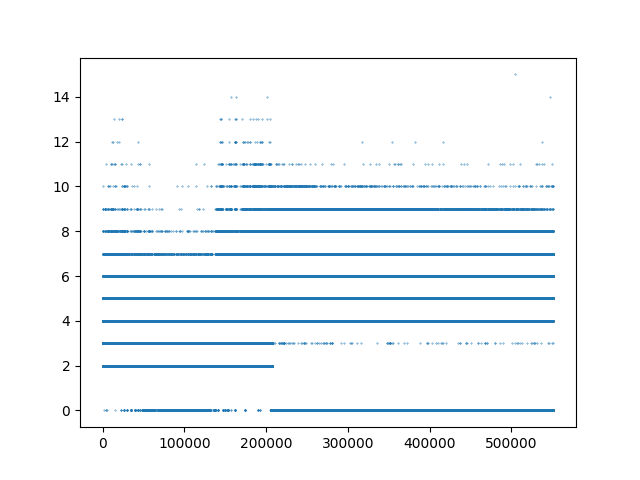
\includegraphics[width=.5\linewidth - 0.25cm]{img/edge_usage/aegaeis-ref-graph.png} }}%
        %\qquad
        \subfloat[\centering{}aegaeis-visibility]{{\includegraphics[width=.5\linewidth - 0.25cm]{img/edge_usage/aegaeis-ref-visibility.png} }}%
    \end{figure}
\end{frame}


\begin{frame}{}
    \begin{figure}[h!]%
        \centering
        \subfloat[\centering{}CH Suchbaum]{{\includegraphics[width=.5\linewidth - 0.25cm]{img/ch_search.png} }}%
        %\qquad
        \subfloat[\centering{}Dijkstra Suchbaum]{{\includegraphics[width=.5\linewidth - 0.25cm]{img/full_dijkstra.png} }}%
    \end{figure}
\end{frame}

\end{document}
